\chapter{Problem description}
% News & generic usage

The goal of Tribler is to become an information sharing platform / video-on-demand platform that protects the privacy of its users and is resilient to attacks while not relying on existing infrastructure.
The goal of this thesis project is to enable all Tribler functionality on mobile Android devices.


\section{Shift to social media}
% Production
Sharing opinion and discussion is enabled on social media.
A global dialog is possible through social media like Twitter, Instagram and Facebook.
% Consumption
People receive local and global news perceived relevant to their group on their social media feed.
Young people in particular are shifting to social media as their number one source. \cite{reuters_social_media}
As shown in this age distribution graph, figure \ref{fig:reuters-news-sources-ages}.
\begin{figure}
	\centering
	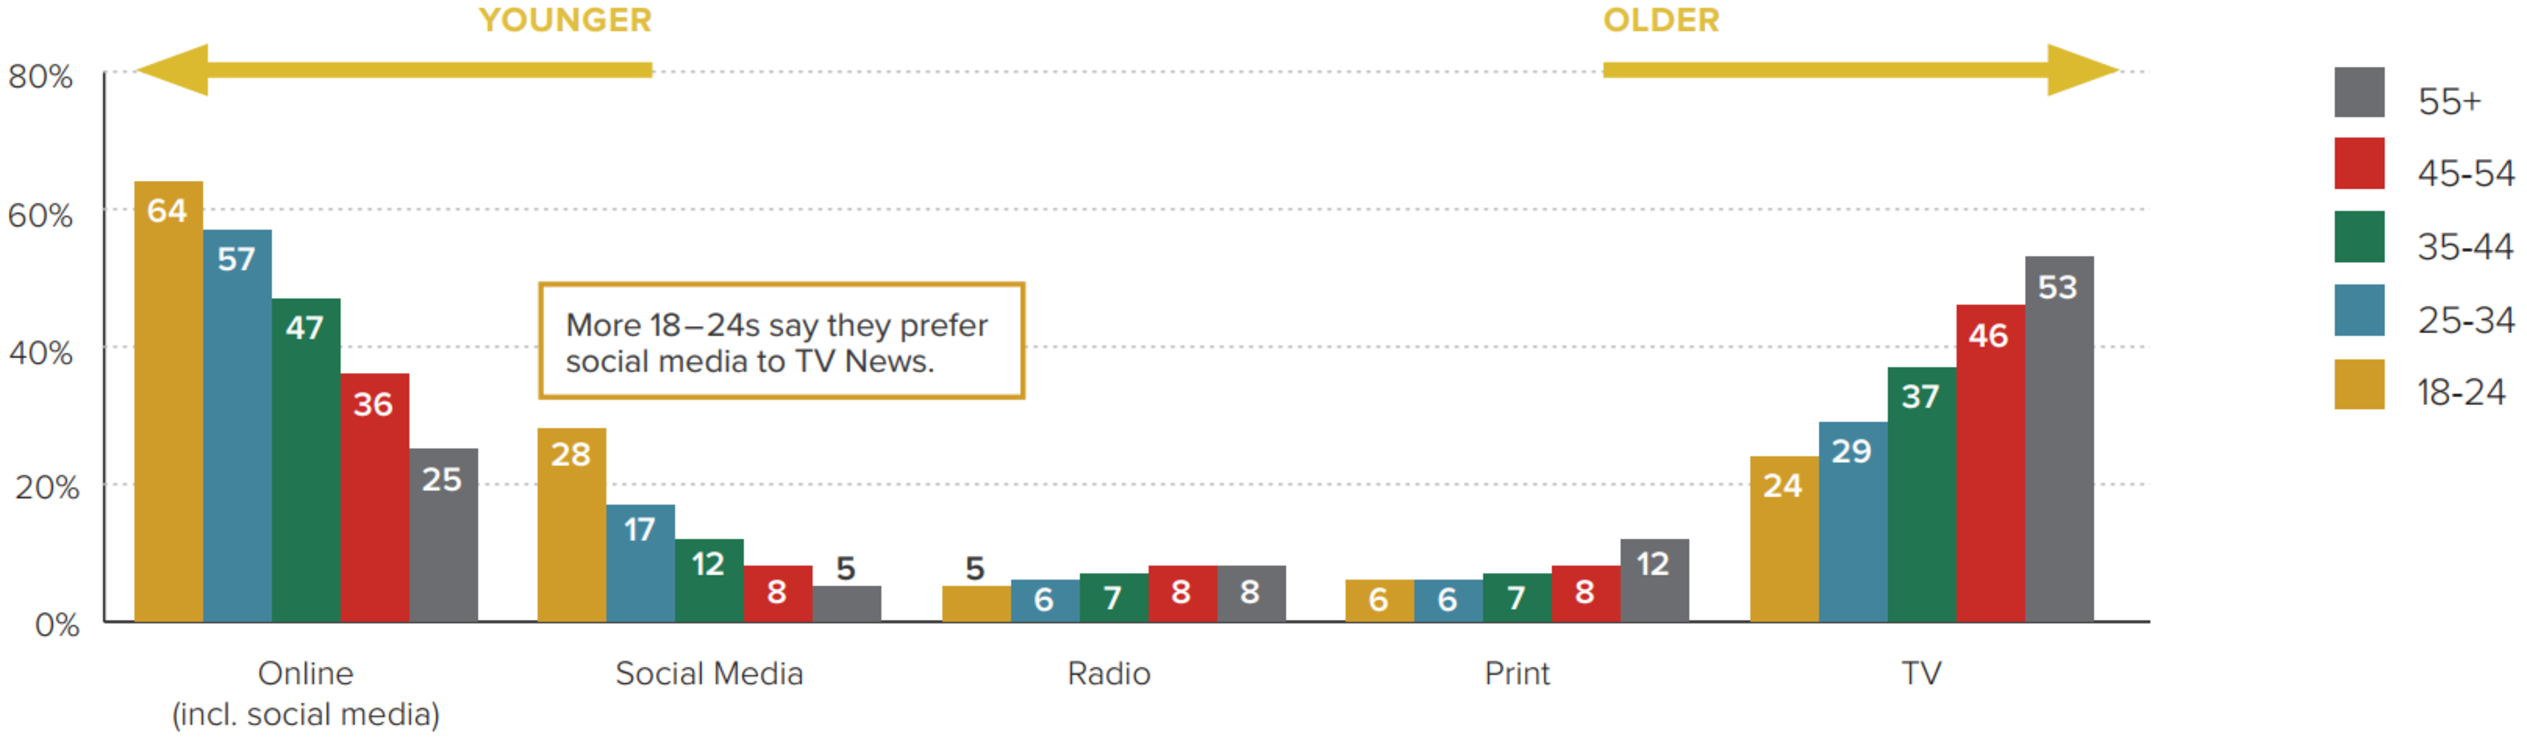
\includegraphics[width=\textwidth]{reuters-news-sources-ages}
	\caption{Main news sources split by age \cite{reuters_social_media}}
	\label{fig:reuters-news-sources-ages}
\end{figure}
% Distribution
Not only is social media more and more becoming a major distribution channel for news, it also starts delivering input for news and story creation.
This way social media has become both the source and outlet for investigative journalism.


\section{Rise of the smart-phone}
% Ubiquity
A smart-phone has the unique property of being a ubiquitous device that is highly mobile and extremely connectible.
The entire world has a smart-phone.
Even or especially areas without traditional infrastructure they are ubiquitous.

The capabilities and versatility of smart-phones enable it to be used for production and consumption of news and social media.
The users themselves are turning from con-sumers into pro-sumers.
% Production
% Distribution
With regards to production most smart-phones have one or more cameras to record multi-media content that can be shared immediately from the device.
Eye-witnesses often have smart-phones at hand to immediately record an event with and post it on social media.
No news desk or professional equipment is necessary to relay news directly from eye-witnesses to the masses anymore.
% Social journalism
People with camera phones can reach millions of people with multi-media in a very short timespan, becoming social journalists.
% Editorial / Journalism / Processing
The ease of reaching a global audience by an individual with a smart-phone diminishes the role of an expert curator handling incoming information.

% Consumption
Also with regard to the consumption medium mobile devices increasingly replace the role of traditional outlets like TV, newspapers and other physical media.


\section{Communication during crisis}
In crisis situations, like natural disaster or unrest, people need to communicate and coordinate their efforts to restore safety.
In this context the smart-phone becomes particularly important because it is often carried on person and provides connectibility.

In recent calamities people could mark themselves as safe on social media, effectively broadcasting that information to all their family and friends on social media instead of contacting them one by one or not at all due to congestion in the communication channels.

However, several natural disasters have taken out the necessary infrastructure on numerous occasions for a prolonged period of time. %katrina

Therefore we require a solution to enable social media on smart-phones that does not require infrastructure. % persistent, established ??


\begin{figure}
	\centering
	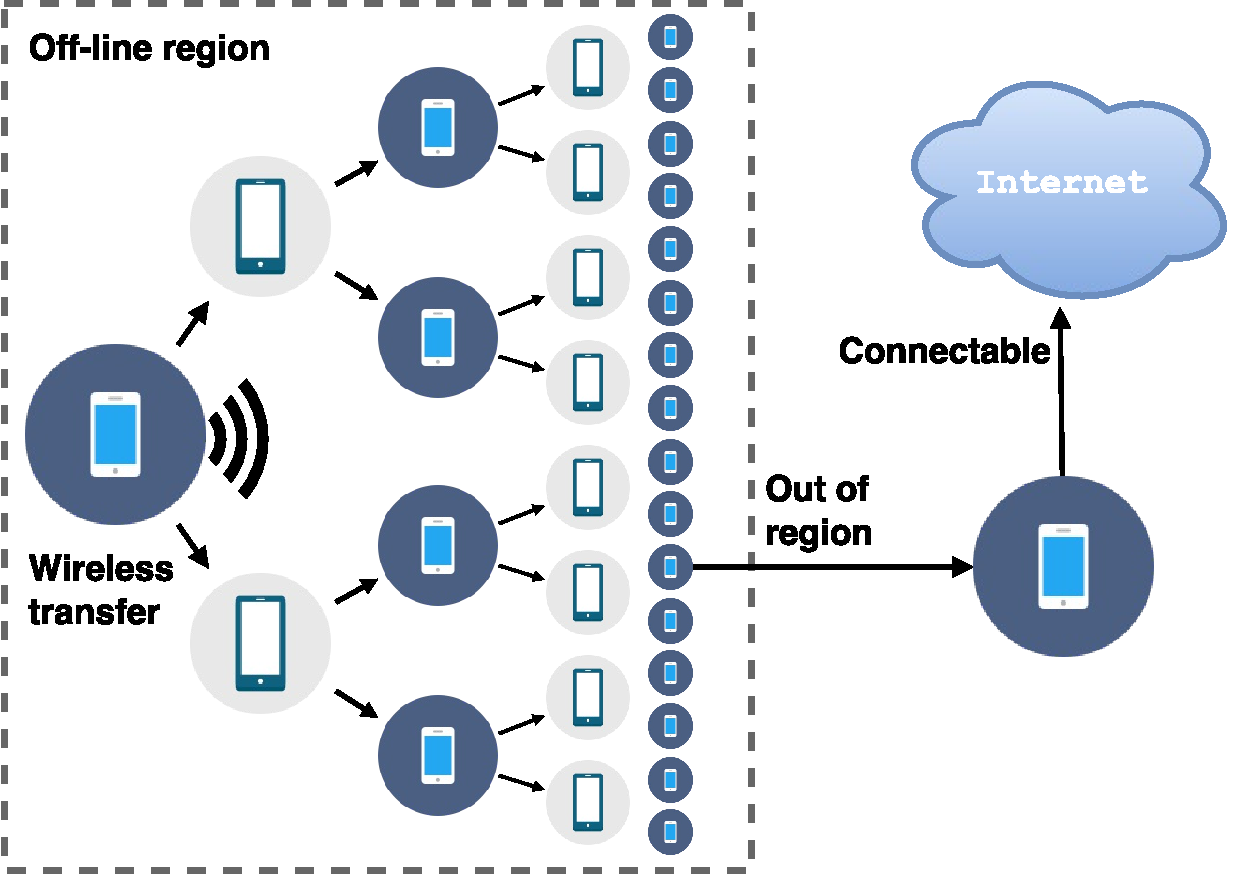
\includegraphics[width=0.7\textwidth]{viral_spreading}
	\caption{Anonymity via proxies}
	\label{fig:viral_spreading}
\end{figure}


\section{Invasion of privacy}
Social media companies use targeted advertisement as part of their business model.
Information considered private by users of social media is actually used to broker targeted advertisements.
Subsequently users can be confronted with their information being misused in various ways beyond their control.
This lack of control over your own privacy can lead to arbitrary interference as defined in UDHR article 12. %ref, example, human rights watch, nelie kroes, etc.
Integration of social media on regular websites makes every page-view and click on these websites traceable to an individual, directly benefiting the business model of targeted advertisements


\section{Censorship}
Pervasive monitoring of digital citizens by Internet providers on behalf of governments to enforce censorship laws raises severe privacy concerns.
% Large scale monitoring
The lack of anonymity becomes a problem when the users privacy is being invaded.
Revealing personal information can be deduced from search queries for example, or associations on social platforms.
When this information can be used for targeted advertising it becomes very valuable, and creates an incentive for the parties that have access to this information to sell it to third parties.
In fact the business model of social media appears to be serving targeted advertisements to its users on behalf of third parties.
What's even worse is social media integrated into regular websites to de-anonymize and track the whereabouts of users even outside of the social media realm.
Whenever users lose control over their privacy it becomes a serious problem.


% Dissent
The incentive to de-anonymize the user, not only causes a lack of privacy, but also a potential lack of freedom of expression, as it hands key information to a censor: who is expressing dissent and who is associated with this person on-line.
Cyber-suppression has become a reality when you no longer can be associated with opinion-makers or foreign journalists on-line.

% Single point of entry
Internet exchange (IX) infrastructures are among the central components in the inter-network architecture that are also vulnerable to monitoring, censorship and Internet kill-switches.
As such, not everyone has unrestricted access to the Internet due to censorship and surveillance.
In fact a significant part of today's Internet users is affected by these attempts to hide or distort reality. %ref
This interference directly affects the universal right to freedom of opinion and expression as stated in article 19 of the Universal Declaration of Human Rights (UDHR).


For example: Arab Spring. Kill switches are real.
What are kill-switches?


Large portions of the global dialog on social media is uncontrolled by traditional media or governments.

Utilizing infrastructure is undesired because of censorship.


The sophistication of censorship techniques is pushed forward by the drive to stay ahead of attempts trying to circumvent it.
Increasingly though, Internet traffic is put under surveillance and obfuscation techniques are targeted by restrictions.


% Adversary model ?

To ensure that no controlling party can exercise censorship authority must be distributed over all users. % creating an \emph{autonomous} system.
If all information is located in one or a few places, the parties in charge of that location will still have control over it, so information must distributed all users as well, creating a \emph{communication} system.

Then if all users want to use this system to share, order and appreciate each others information, in other words the essence of social media: social interaction, with everyone being able to interact in the same way, we need to  distribute functionality over all users, creating a \emph{cooperation} system.


\section{Distributed solutions}
% Solution
Fully distributed systems capture these characteristics.
To render the effect mute of the Internet kill switches in existence shown to be used we propose a distributed solution.
Without any central component in the system it is no longer susceptible to censorship without everyone participating.
Leveraging the properties of mobile devices, like smart-phones as stated above, together with the features of Tribler we see a perfect match.
Because censorship and large scale monitoring is difficult in decentralized networks our proposed solution can work in these situations.

% Eindig aantal servers points of failures
Networks that are not fully decentralized can be disrupted by taking down a limited number of nodes, less than the total number of nodes.
Thanks to a server-less design we can say:
The only way to take Tribler down is to take the entire Internet down.

Mobile devices are essential to take the next step in the face of censorship.
If we can use smart-phones to create a fully decentralized social network we can say:
The only way to take Tribler down is to take everybody's smart-phones away.

The importance of mobile devices in this context is crucial , if we want to do even better in spreading information, which is not been done before, we surmount than next hurdle.

Peer-to-peer communication technology is essential for a server-less distributed system.
Mobile devices typically do not require infrastructure to exchange information, like those equipped with Bluetooth or capable of ad hoc Wi-Fi.
Smart phones are ubiquitous everywhere in the world and used to access social media and retrieve information from the Internet.
Fortuitously these are also the type of mobile devices that can communicate peer-to-peer.

Example: Arab spring \cite{Johan_2001}


% Fragmented
Various initiatives have been started to deal with one or both of these problems. \cite{re_decentralize}
%FIG? From re-decentralized: top projects that match/compare.

\begin{figure}
	\centering
	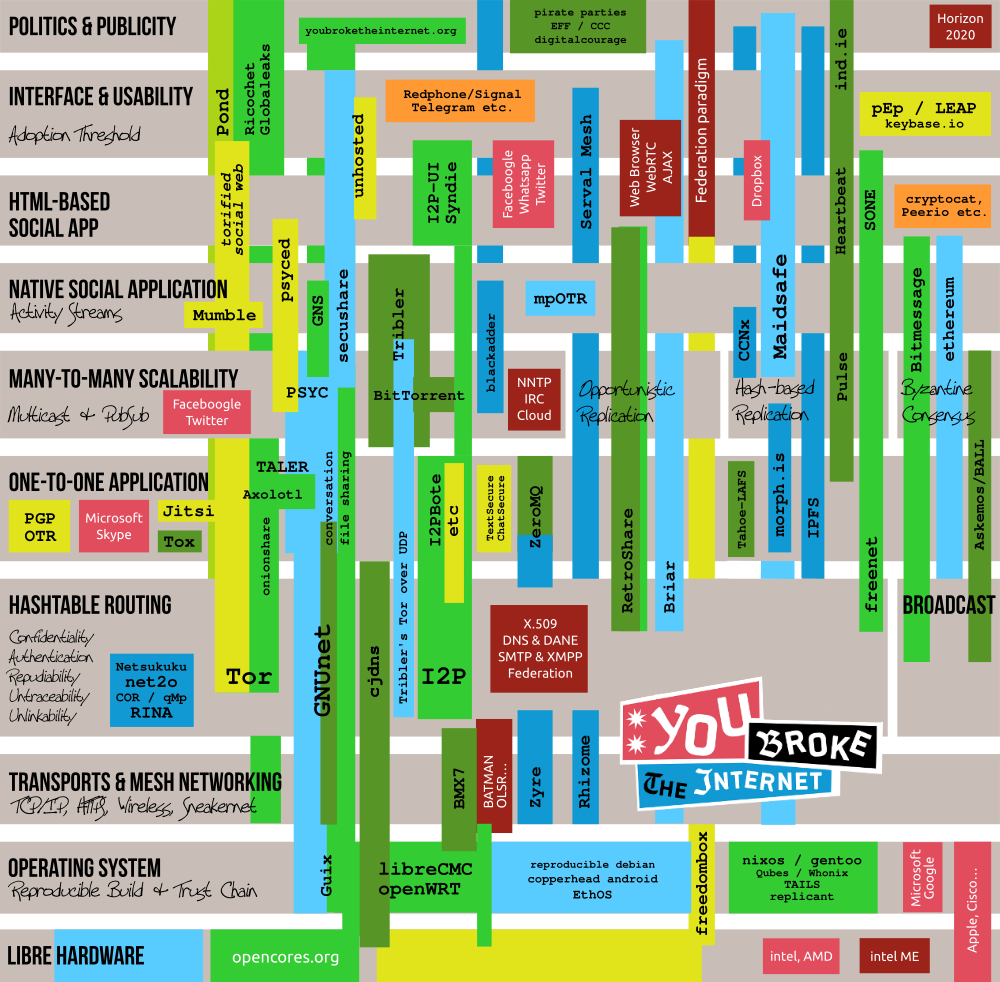
\includegraphics[width=\textwidth]{youbroketheinternet}
	\caption{Source: www.youbroketheinternet.org}
	\label{fig:youbroketheinternet}
\end{figure}

Figure \ref{fig:youbroketheinternet} shows a mapping of projects that are or have been working on that.
The fragmentation is clear from the figure.
There are a few big players, as can be seen from the figure, but none of them provide a full solution.

%potential skip:
%being first
%engineering perfection
%time to market
%popularity
%make a difference
%Tribler mobile vs periscope
%fully functional prototype, but poor user interface (unpolished)
%real world impact proven insufficient
%we want to change the world implicit


%\section{Define alternatives} %design space %solution space
%\cite{https://www.ietf.org/mail-archive/web/ietf-privacy/current/msg00215.html}
% why existing technology is not sufficient to
% meet the described demands. The example proposed was the tor onion
% network in combination with XMPP or the orbot smartphone app. After
% much discussion the conclusion was that existing technologies, such as
% tor facilitate protected point-to-point communication. However,
% possible desired use cases focus more on current Twitter-like social
% media practices, best typified as a "global conversation".
% Furthermore, current social media revolves around video-rich,
% real-time interaction with groups, hashtag-based discovery and social
% networking. All of these aspects are not offered or are incompatible
% with current-generation of privacy enhancing technology



% Refereren aan eigen werk versplintering in oplossingen
There is no de-facto solution available on mobile platforms. \cite{literature_survey}
Previous research has shown that there is no solution that solves the problem entirely in a sustainable way.
Tribler is our attempt to solve this problem entirely in a sustainable way.
To see if it is feasible to apply it in a mobile context as described above, we need to port it.

% Previous Tribler-mobile app's
Previous attempts failed to deliver all functionality. \cite{bsc_1,2,3}
Maintainability issues with earlier designs were a large part of the reasons why.
We changed the architecture of Tribler for our approach.

\section{Contributions}
The main contributions of this thesis are making Tribler available on mobile devices.
By doing that all research with regard to the problems that Tribler tries to solve becomes possible on the mobile platform.
And the resilience of Tribler against attacks on the Internet is greatly increased.

